\chapter{Fundamentação Teórica}

Em uma destilação batelada a medida que o tempo passa, o liquido do vaporizador fica mais pobre no componente mais volátil e mais rico no componente menos volátil por meio de sucessivas condensações e vaporizações que ocorrem dentro da coluna, especialmente na zona de recheio.

\subsection{Hipóteses adotadas:}

\begin{itemize}
	\item Abordagem simplificada, admitindo simplificações do Método McCabe-Thiele;
	\item Retenções de material nos pratos da coluno (Hold up's) foram desprezadas;
	\item Taxas de vaporização constante;
	\item Equilíbrio Líquido Vapor entre o líquido no vaporizador e o vapor gerado no mesmo instante.
\end{itemize}


\subsection{Parâmetros}

\begin{itemize}
	\item \emph{t}: tempo;
	\item \emph{B(t)}: número de moles de líquido no vaporizador no instante t
	\item \emph{$B_{0}$}: valor de B(t) no instante t=0;
	\item \emph{$X_{B}(t)$}: fração molar do componente no instante t no vaporizador;
	\item \emph{$X_{B0}$}: fração molar do componente no instante t=0 no vaporizador;
	\item \emph{ D(t): }Vazão do destilado no instante t;
	\item \emph{$X_{D}(t)$}: fração molar do destilado no instante t;
	\item \emph{$X_{P}(t)$}: fração média do componente no tanque de produto no instante t (acumulado até o tempo t).
%	\item \emph{}
%	\item \emph{}
\end{itemize}


\subsection{Modelagem Matemática}


\begin{figure}[H]
	\begin{center}
		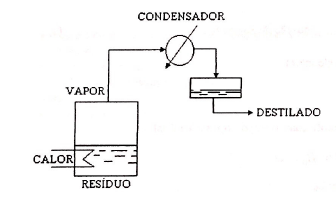
\includegraphics[scale=0.7,trim={0cm -9 0 0}]{figuras/ladeq/destil/modelo}
		\vspace{-20pt}
		\caption{Modelo de destilador de batelada.}
		\label{ladeq/batelada}
	\end{center}
\end{figure}

Equações:


\begin{equation}\label{eq1}
\frac{\mathrm{d} }{\mathrm{d} t}(Bx_{B}) = -Dx_{D}
\end{equation}

\begin{equation}\label{eq2}
x_{B} \frac{\mathrm{d} }{\mathrm{d} t}B + B\frac{\mathrm{d} }{\mathrm{d} t}x_{B} = -Dx_{D}
\end{equation}

\begin{equation}\label{eq3}
x_{B} \mathrm{d} B + B \mathrm{d} x_{B} = -Dx_{D}\mathrm{d}t
\end{equation}

\begin{equation}\label{eq4}
D = -\frac{\mathrm{d} }{\mathrm{d} t}B \rightarrow D \mathrm{d} t = -\mathrm{d} B
\end{equation}

Substituindo \ref{eq4} em \ref{eq3}:

\begin{equation}\label{eq5}
x_{B}\mathrm{d} B + B \mathrm{d} x_{B} = x_{D} \mathrm{d}B
\end{equation}

Rearranjando a equação \ref{eq5}
\begin{equation}\label{eq6}
(x_{B} - x_{D}) \mathrm{d}B = - B\mathrm{d} x_{B}
\end{equation}

\begin{equation}\label{eq7}
(x_{D} - x_{B}) \mathrm{d}B = B\mathrm{d} x_{B}
\end{equation}

Separando as variáveis:

\begin{equation}\label{eq8}
\frac{\mathrm{d} B}{B} = \frac{\mathrm{d} x_{B}}{(x_{D} - x_{B})}
\end{equation}

Fazendo a integral do tempo 0 até um determinado tempo t:

\begin{equation}\label{eq9}
\int_{B_{0}}^{B} \frac{\mathrm{d}B}{B} = \int_{B_{0}}^{B} \frac{\mathrm{d}x_{B}}{(x_{D} - x_{B})}
\end{equation}


Equação \ref{eq10} também é conhecida como Equação de Rayleigh:

\begin{equation}\label{eq10}
\ln (\frac{B}{B_{0}}) = \int_{x_{B0}}^{x_{B}} \frac{\mathrm{d}x_{B}}{(x_{D} - x_{B})}
\end{equation}

Se integramos o balanço global (\ref{eq4}):

\begin{equation}\label{eq11}
\int_{0}^{t} D \mathrm{d}t = \int_{B_{0}}^{B} -\mathrm{d}B
\end{equation}

Sabendo-se que D é constante com o tempo, suposição inicial:

\begin{equation}\label{eq12}
-D t = B - B_{0} \rightarrow B = B_{0} - Dt
\end{equation}

Divide-se a equação \ref{eq11} por $B_{0}$:

\begin{equation}\label{eq13}
\frac{B}{B_{0}} = 1 - \frac{Dt}{B_{0}}
\end{equation}


Tempo de Batelada:

\begin{equation}\label{eq14}
t = \frac{B_{0}}{D} \left \{ 1 - \exp \left ( \int_{x_{B0}}^{x_{B}}  \frac{\mathrm{d} x_{B}}{(x_{D}-x_{B})} \right ) \right \}
\end{equation}

Balanço de massa por componente no instante t:

\begin{equation}\label{eq15}
B_{0} x_{B0} = B(t)x_{B}(t) + (B_{0} - B(t))x_{p}t
\end{equation}

\begin{equation}\label{eq16}
x_{p}(t) = \frac{ x_{B0} - \frac{B(t)}{B_{0}} x_{B}(t) }{t - \frac{B(t)}{B_{0}}}
\end{equation}

\begin{equation}\label{eq17}
x_{p}(t) \frac{ x_{B0} - x_{B} \exp \int_{x_{B0}}^{x_{B}} \frac{\mathrm{d} x_{B}}{(x_{D}(t) - x_{B}(t))}}{1 -  \exp \int_{x_{B0}}^{x_{B}} \frac{\mathrm{d} x_{B}}{(x_{D}(t) - x_{B}(t))}}
\end{equation}






